%情報処理学会全国大会原稿テンプレート ver. 1.2

\documentclass[uplatex,twocolumn]{jsarticle}
\usepackage[top=30mm,bottom=25mm,left=20mm,right=20mm]{geometry}
\usepackage[T1]{fontenc}
\usepackage{txfonts}
\usepackage[expert,deluxe]{otf}
\usepackage[dvipdfmx,hiresbb]{graphicx}
\usepackage[dvipdfm]{hyperref}
\usepackage{pxjahyper}
\usepackage{multicol}
\setlength{\columnsep}{7mm}

\title{\vspace{-10mm}クラウドファンディングにおける成功の判別分析\footnotemark[0]}%要修正
\author{\large{三浦 泰介\footnotemark[2]\qquad 矢吹 太朗}\\千葉工業大学 社会システム科学部 プロジェクトマネジメント学科\footnotemark[3]}%要修正
\date{}
\pagestyle{empty}
\begin{document}
\twocolumn[\maketitle]

\begingroup
\def\thefootnote{\fnsymbol{footnote}}
\footnotetext[0]{欧文タイトル.}%要修正(最後はピリオド)
\footnotetext[2]{Firstname Lastname (\verb|MAIL|)}%要修正
\footnotetext[3]{Department of Project Management, Faculty of Social Systems Science, Chiba Institute of Technology.}
\endgroup

\section{序論}
クラウドファンディング\cite{wiki}が世界中で利用されている.\cite{kaihatu}
クラウドファンディングとは,プロジェクトの活動資金を,インターネットを利用し,不特定多数の支援者から募集する資金調達の手法で,個人規模の小さなプロジェクトでも利用できるため,ベンチャー企業や学生から注目されている.

クラウドファンディングは窓口となるウェブサービス上で実施されるのが一般的であり,日本ではMakuake(\url{https://www.makuake.com/})やREADYFOR(\url{https://readyfor.jp/})の利用者数が多い.

クラウドファンディングは一般的に資金提供者に対するリターンの形態によって以下の3つに分けられる.

\begin{description}
\item[寄付型] 金銭的リターンのない
\item[投資型] 金銭的リターンのある
\item[購入型] 権利や物品を購入することで支援する
\end{description}

日本におけるクラウドファンディングは,2014年に金融商品取引法が改正されるまで\cite{kisei}は,見返りを得ない寄付型,購入型に限られていた.購入型はリターンがあるためリターンを目当てに多くの出資者が集まる傾向があり,購入型は日本で一番市場が大きいクラウドファンディングの形態である.

クラウドファンディングに出資する場合には,ウェブサイトから支援したいプロジェクト毎に決められた支援コースを選択し,金額を支払うことで行える.
クラウドファンディングが失敗した場合は,払った金額は返金される.





\section{目的}
プロジェクトにおいて資金集めは重要で,資金集めができなければプロジェクトは破綻してしまう.
期間内に資金が集まれば資金調達は成功,集まらなければ失敗である.
そのため,クラウドファンディングを利用する場合は,プロジェクト自体を成功させる前に,クラウドファンディングを成功させなければならない.

そこで本研究では,クラウドファンディングの成功要因を分析する.
クラウドファンディングでは,プロジェクトの内容以外にも,出資金額や出資方法の選択肢など,資金調達の成功に関わると思われる要因が複数ある.
クラウドファンディングの事例を収集し,これらのさまざまな要因と資金調達の結果(成否)の関係を分析することで,プロジェクトの内容とは別に,クラウドファンディングの成否に関わる要因を見いだすことを目指す.

\section{手法}
クラウドファンディングの成功要因を以下の手順で分析する.

まず,日本の大手クラウドファンディングサービスであるMakuakeとREADYFORを定期的(1日1回)チェックし,そこで実施されているクラウドファンディングについての情報を収集する.収集する情報は,目標金額と支援コース数,支援最低金額,支援最高金額,資金提供者が得る物,動画の有無である.最終的に資金調達に成功したかどうかも記録する.

次に,資金調達の成否の決定木を作成する.決定木の目的変数は資金調達の成否,説明変数は上述の収集情報(目標金額等)である.

最後に,作成された決定木をもとに,クラウドファンディングの成功要因を考察する.

\section{結果}

\begin{figure}
\centering
\includegraphics[width=\textwidth]{figure.eps}
\caption{クラウドファンディングの成否の決定木(要因は「手法」に掲載)}\label{決定木}
\end{figure}

100個のプロジェクトのデータを収集し,決定木分析を行った.使用した要因は「手法」で述べたとおりである.作成した決定木は図\ref{決定木}のとおりである.この決定木は,全体の83\%を再現している.

分析に用いる要因に,そのプロジェクトに対して付けられたFacebookの「いいね」の数と,そのプロジェクトのURLがTwitterでつぶやかれた回数を加えた場合の決定木が図\ref{決定木2}である.

\begin{figure}[htb]
\includegraphics[width=\columnwidth,clip]{figure2.eps}
\caption{分析要因に「いいね」の数とつぶやきの数を加えた場合の決定木}\label{決定木2}
\end{figure}

\section{考察}

図\ref{決定木}の決定木から,支援最低金額が3,744円から35,990円で目標金額が375,000円以上のプロジェクトの成功率が最も高くなることがわかる.
これは支援最低金額でリターンがもらえるプロジェクトが成功しやすいのではないかと考えられる.支援最低金額が500円や1000円のコースは,お礼のメールや手紙が届くものが多いが,支援最低金額が3000円や5000円程度の額であると音楽家のCDや出版物であればリターンをもらえるものが多く,リターンを目当てにした支援者が多いことが伺える..

目標金額が375000円以上のプロジェクトの成功率が高くなることは,目標金額が375000円という設定が今回使用した100件の目標金額の平均である1606724円よりもおよそ4分の1程度の低く,目標金額設定が低いと支援者としてもクラウドファンディングが成功しやすいと考えて支援するのではないかと推察できる.

また決定木に出てくる要因の頻度として最低金額と目標金額が頻繁に出てくることからもこの2つの設定額が重要であることが推測できる.

目標金額が著しく高いプロジェクトは失敗しているものが多く見られる.目標金額が高い場合多くの支援者を集める必要があり,日本においてクラウドファンディングの利用者が海外に比べると少なく,多くの支援者数を集めることが困難であることが考えられる.

Facebookの「いいね」ボタンやTwitterの「ツイート」ボタンを利用された数が大きいプロジェクトは成功している傾向にあり,SNSで広報を積極的に行うことが成功に繋がると考えられる.この2つの要因は自分で意図的に操作することは難しいがSNSを通してプロジェクトの進捗状況を報告したり,SNSでの反応に対して対応をすることで数を増やすことは多少可能であり,操作までとは言えないものの伸ばす努力は十分に可能であると考えられる.

\section{結論}
本研究では,決定木を書くことでクラウドファンディングにおける重要な要因を見つけることができた.調査要因やデータが少ないことは否めないが,成功合否に関わる要因をこの手法で探し出すことで可能である.

また成功合否の一致率が83\%であることから今回作成した決定木は十分使えるものであると考えられる.

\bibliographystyle{junsrt}
\bibliography{biblio}%「biblio.bib」というファイルが必要.

\end{document}
